In this section, we introduce the Hazel stepper filter.

We recognized some key capabilities that traditional debuggers have and will be
also helpful to a debugger for functional programming languages.
\begin{enumerate}
  \item Evaluation can be paused at some point and resumed later. The user
    should be able specify where/when the evaluation should be paused. This is
    usually implemented as the breakpoint mechanism in a traditional debugger.
  \item Paused evaluation can be stepped through. traditionally, debuggers will
    provide user with three buttons to ``step through'', ``step over'' and
    ``step out''.
\end{enumerate}

Moreover, we want some extra capabilities that are specific to functional
programming languages and a classroom settings, especially Hazel, to be a
useful tool for teaching and learning functional programming.
\begin{enumerate}
  \item It can skip the stepping process of some \emph{kind} of expression.
  \item It controls the evaluation of the program in a granularity of
  expression, instead of a granularity of line or instruction.ß
\end{enumerate}

To serve as a good tool for understanding the behavior of a program, the stepper
filter should have consistent behavior with the semantics of the language. Hazel
internally uses a environment-based big-step evaluator to evaluate the program,
but it has a consistent behavior with the substitution-based one. Therefore,
the stepper filter shall not exhibit different behavior when building upon a
environment-based evaluator or a substitution-based evaluator.

The evaluation order of Hazel is not specified. Therefore, an expression that is
not value might have multiple possible choice 

\subsection{Matching}


Terms that has the same structural form after substituting all bounded variables
are considered \emph{matched}.

\begin{verbatim}
let x = 3 in
eval x + 3 in
x + 3
\end{verbatim}
shall has the same behavior as the program
\begin{verbatim}
let x = 3 in
eval 3 + 3 in
3 + 3
\end{verbatim}

\begin{verbatim}
eval $e in
let g = fun x -> x + x in
pause g($v) in # or pause (fun x -> x + x)($v) in
(fun x -> x + x)(3)
== (fun x -> x + x)(3) # or g(3) #
\end{verbatim}

\begin{figure}[h]
  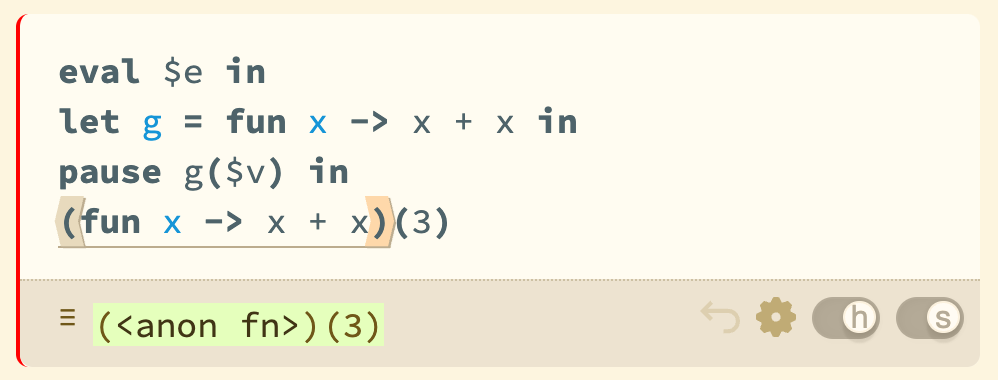
\includegraphics[width=0.4\textwidth]{images/match-mod-subst.png}
\end{figure}

As in a substitution-based evaluator, the substitution is applied to the
the body of a function:
\begin{verbatim}
eval $e in
let y = fun x -> x in
let h = fun x -> (fun y -> y) in
pause (fun x -> y)($v) in
h(3)
== h(3) # or (fun x -> (fun x -> x))(3) #
\end{verbatim}

\begin{figure}[h]
  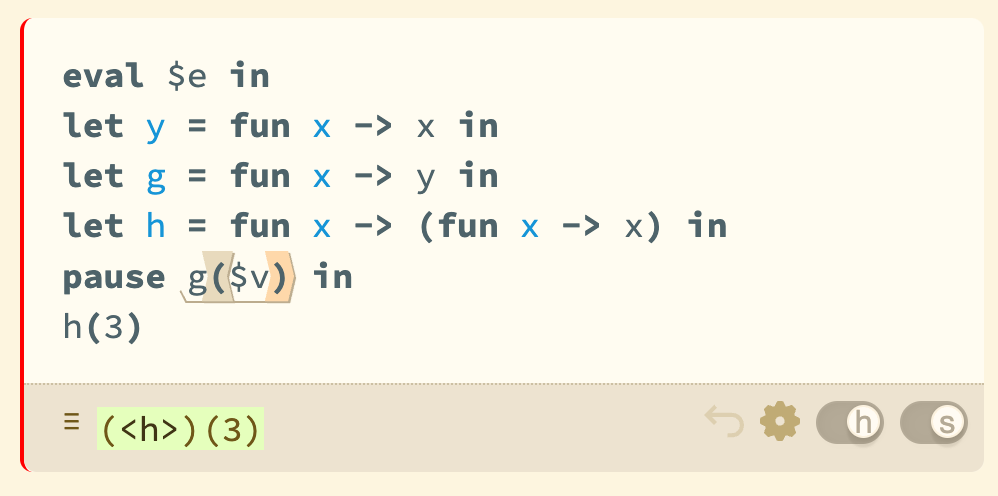
\includegraphics[width=0.4\textwidth]{images/match-recursive.png}
\end{figure}

A immediate corollary of this is that the stepper filter shows that
the filter cannot be applied to a variable, since the substitution is always
performed ahead of the matching process, and for the filter it shall not be
able to match against a variable.

\begin{verbatim}
eval $e in
let x = 3 in
pause x in
x + x
== 6
\end{verbatim}

\TODO{Discuss: whether or not to use alpha-equivalence here.}

\subsection{Four filters: Hide, Eval, Pause and Debug}

\TODO{Discuss: mention skip all, skip one, pause all and all one?}

Typical use case for the four basic filters.

\paragraph{eval} We want to use the \verb|eval| to \emph{evaluate} all sub-expressions that matches the pattern.
\begin{verbatim}
eval 1 + 2 in
1 + 2
== 3
\end{verbatim}

We want the \verb|hide| filters to hide away one step.
\begin{verbatim}
hide let   =   in   in
let x = 3 in
let y = 4 in
x + y
== 3 + 4
== 7
\end{verbatim}
while using \verb|eval| it will behave like this:
\begin{verbatim}
eval let   =   in   in
let x = 3 in
let y = 4 in
x + y
== 7
\end{verbatim}

\paragraph{hide} The \verb|hide| filter will be \emph{used up} when its body
expression is actually being evaluated.

During evaluation, we want to be able to examine every instruction
transitioning steps.

\begin{verbatim}
eval 1 + 2 + 3 + 4 in
pause 3 + 3 in
1 + 2 + 3 + 4
== 3 + 3 + 4
== 10
\end{verbatim}

This would be especially useful when unfolding a higher level
expression to its individual terms, for example I want to know how
many terms of \verb|fib(1)| I need to call to evaluate the whole
\verb|fib(5)|.

On the other hand, we want to went through all the evaluation process of a
sub-expression, for example when debugging the implementation of a function
\begin{verbatim}
let (is_even: Int -> Bool, is_odd: Int -> Bool) = ... in
debug is_odd($v) in
is_even(5)
\end{verbatim}

The difference between \verb|pause| and \verb|debug| is subtle. For
example, considering the following two piece of code:
\begin{verbatim}
eval $e in
pause (1 + 2) + (3 + 4) + (5 + 6) in
eval 3 + 7 + (5 + 6) in
(1 + 2) + (3 + 4) + (5 + 6)
== (1 + 2) + (3 + 4) + (5 + 6)
== 21
\end{verbatim}
and
\begin{verbatim}
eval $e in
debug (1 + 2) + (3 + 4) + (5 + 6) in
eval 3 + 7 + (5 + 6) in
(1 + 2) + (3 + 4) + (5 + 6)
== (1 + 2) + (3 + 4) + (5 + 6)
== 3 + (3 + 4) + (5 + 6)
== 21
\end{verbatim}
The first one will immediately evaluate to final value is because it is a \verb|pause| statement, which will be only effective once.

Filters can't be applied on values. A more significant corollary of this is they cannot be applied on variables as well.
\begin{verbatim}
eval $e in
pause x in
pause y in
let x = 3 in
let y = 4 in
x + y
== 7
\end{verbatim}

\subsection{Interaction between filter statements}

\TODO{Q: Do we need formalise these properties?}

We want nested filter statements to behave correctly, i.e.
\begin{enumerate}
\item For every pattern \verb|p|, \verb|pause p| cancels the effects
  of \verb|eval p| and \verb|hide p|, vice versa.
\item Inner filter statements take precedences.
\end{enumerate}

\begin{verbatim}
pause 1 + 2 + 3 + 4 in
eval 1 + 2 + 3 + 4 in
1 + 2 + 3 + 4
== 10
\end{verbatim}

\begin{verbatim}
pause $e in
eval 1 + 2 + 3 + 4 in
pause 1 + 2 + 3 + 4 in
1 + 2 + 3 + 4
== 1 + 2 + 3 + 4
\end{verbatim}

\begin{verbatim}
pause $e in
hide (let   =   in  ) in
pause (let   =   in  ) in
let x = 3 in
x + 4
== let x = 3 in x + 4
\end{verbatim}

The nesting properties should works across bindings.

\begin{verbatim}
eval $e in
let x = 1 in
pause 3 + 3 in
let y = 2 in
eval 3 + 3 in
x + y + 3 + 4
== 10
\end{verbatim}

\begin{verbatim}
let add = fun x, y -> pause $e in x + y in
eval $e in
add(3, 4)
== [3 + 4]
\end{verbatim}

We want the filter to recover to \emph{older} state when it finish
evaluating matched sub-expression.

\begin{verbatim}
pause $e in
eval 1 + 2 + 3 + 4 in
pause 3 + 3 in
1 + 2 + 3 + 4
== 3 + 3 + 4
== 10
\end{verbatim}

After evaluating \verb|3 + 3|, the stepper falls back to eval mode
since eval filter matches \verb|1 + 2 + 3 + 4|, so it directly
evaluates to \verb|10|.

We also want a \verb|eval| filter to automatically evaluate all sub-expression
until it cannot proceed.

\subsection{Handling inconsistency between DHExp and UExp}

\TODO{Discuss: Move to implementation.tex?}

There are inconsistencies between the surface expression and expression for
evaluation in Hazel. For example, fix-points are inserted in the expression
during elaboration. We want the filters to work with fix-points, with-out user
acknowledging that they actually needs a fix-point to implement the recursion.

\begin{verbatim}
let map : ([Int], Int -> Int) -> [Int] = fun xs, f ->
  case xs
  | [] => []
  | hd :: tl => f(hd)::map(tl, f)
  end
in
let square = fun x -> x * x in
pause map($v) in
map([1, 2, 3], square)
== 1::map([2, 3], f)
== 1::4::map([3], f)
\end{verbatim}

In the example above, we don't want to use to click twice to do unroll and apply, instead we want to merge these two transition
in one step.

\subsection{Good but unrealistic for now}

\TODO{Discuss: Is it better remove in total?}

There are also something that we think would be intuitive and useful but not possible with current implementation

\begin{verbatim}
let fib : Int -> Int =
  fun n ->
    if n <= 1 then
      n
    else
      fib(n - 1) + fib(n - 2)
in
pause fib($v) + fib($v) in
fib(5)
== 3
\end{verbatim}

Intuitively we shall see a evaluation trace like this:
\begin{verbatim}
...
== fib(4) + fib(3)
== fib(3) + fib(2) + fib(3)
== fib(3) + fib(2) + fib(2) + fib(1)
== ...
\end{verbatim}

This is no possible since this require us to traverse all possible
evaluation sequence given a program, which would be super powerful,
but at the same time super slow.

%%% Local Variables:
%%% mode: latex
%%% TeX-master: "main"
%%% End:
